%%%% IJCAI-ECAI-26 preprint -- Week 2
%%%%
%%%% BUILD:  pdflatex main && bibtex main && pdflatex main && pdflatex main
%%%% Needs ijcai26.sty and named.bst alongside this file (both gitignored --
%%%% they come from the official author kit and are not redistributed here).
%%%%
%%%% Figures are rebuilt with: python figures/make_figures.py
%%%% Every number in this paper is produced by a script in experiments/ and
%%%% written to results/. Nothing is typed in by hand.

\documentclass{article}
\pdfpagewidth=8.5in
\pdfpageheight=11in

\usepackage{ijcai26}

\usepackage{times}
\usepackage{soul}
\usepackage{url}
\usepackage[hidelinks]{hyperref}
\usepackage[utf8]{inputenc}
\usepackage[small]{caption}
\usepackage{graphicx}
\usepackage{amsmath}
\usepackage{amsthm}
\usepackage{booktabs}
\usepackage{tikz}
\usetikzlibrary{arrows.meta,positioning,fit,backgrounds}

\urlstyle{same}

\pdfinfo{
/TemplateVersion (IJCAI.2026.0)
}

\title{What an Agent Should Ask, and What It Should Pay:\\Belief, Information Value and Cost in Secret-Scanner Triage}

\author{
Grishma M\\
\emails
grishma.renuka@gmail.com
}

\begin{document}

\maketitle

\begin{abstract}
A secret scanner reports that a string in a repository looks like an API key.
Whether that string still authenticates cannot be established without using it,
and using a credential found in a repository is not permitted. Week~1 of this
project built a cost-derived triage policy for that decision. This paper adds
what the policy was missing: a belief over five states rather than three, an
explicit price on every question the agent could ask, and a rule for when to stop
asking. Three results are not what I expected. First, ranking evidence by
information and by expected cost saved produces near-opposite orders, and the
agent buys evidence exactly where its two free features contradict each other
rather than where a finding looks most severe. Second, a cost of 2400 minutes for
dismissing a live key contained an unstated probability of exploitation equal to
one. Correcting it, together with two other fixes, took recall on hard-coded
fakes from 0.000 to $0.95 \pm 0.02$ while total cost moved by 1.3 minutes---a
failure that cost reporting alone cannot see, because the metric barely moved
while three of five states went from unreachable to reachable. Third, the Week~1 invariance---that free features carry exactly zero
bits about live versus revoked---is a property of the credential format rather
than of secret scanning, and moving the agent to a credential that exposes a
public identifier does not remove the invariance but relocates it onto a
different pair of states, where it is worth 0.0000 bits again.
\end{abstract}

% =====================================================================
\section{Introduction}

A scanner reads a repository and reports that some string in it looks like a key.
That is the whole input. It does not say what kind of key, and it does not say
whether the key works.

The obvious way to find out is to try the key. That is not available to me. I am
not going to authenticate against a third party's API with a credential I found
in someone's repository, and no security team I have spoken to would authorise
it. So the agent has to decide what to do about a string whose most
decision-relevant property it is forbidden to observe.

\paragraph{Scope: private and internal repositories.}
A reasonable first reaction is that a key in a private repository does not
matter. It does. A private repository at a mid-sized company is readable by every
employee with access, every contractor whose access was never revoked, and every
CI runner, scanner and editor integration holding a token; the string is in the
git history of every clone anyone ever made; repositories change visibility when
projects are open-sourced, acquired or mis-forked; and a hard-coded credential is
an audit finding regardless of who can see the repository.

More importantly for this paper, the private case is the \emph{unsolved} one. On
a public repository, GitHub's partner programme notifies the provider and the key
is revoked without anyone deciding anything. Privately, nobody is notified, no
validity check runs, and the agent is left with the problem this paper is about.
That choice of scope turns out to matter more than I understood when I made it,
and Section~\ref{sec:general} measures how much.

\paragraph{Why an LLM answer is not sufficient.}
Asked whether a given string is a live credential, a language model will produce
a confident answer. It has no access to the fact in question. What it can do is
pattern-match the string and its surroundings, which is the evidence the agent
already has for free, and return it as a posterior rather than as a likelihood.
The failure that produces is not being wrong; it is being confidently wrong in a
way that removes the one control---escalation to a person---that would have
caught the mistake.

\paragraph{The narrowed question.}
\begin{quote}
\emph{When a scanner reports a possible credential, which check should the agent
run next, and at what belief should it stop checking and act?}
\end{quote}

\paragraph{Contributions.}
\begin{itemize}
\item A five-state belief model for scanner findings, with the two states Week~1
identified but could not characterise, and a measurement of what each was worth
(Sections~\ref{sec:prob}--\ref{sec:info}).
\item A pricing of every question the agent could ask in minutes rather than
bits, and the resulting purchase behaviour, which is not the behaviour a severity
queue would produce (Section~\ref{sec:select}).
\item A failure that overall cost could not see: an unstated exploitation
probability inside a cost cell (Section~\ref{sec:failure}).
\item A generalisation result: the project's headline invariance is a property of
credential formats, and relocating rather than disappearing when the format
changes (Section~\ref{sec:general}).
\end{itemize}

% =====================================================================
\section{The Same Question, Without the Domain}
\label{sec:umbrella}

Before any of the machinery, the whole design in four numbers.

There is a 35\% chance of rain. Should I carry an umbrella? Costs in units of
annoyance, and they are assumptions:

\begin{center}
\small
\begin{tabular}{@{}lrrr@{}}
\toprule
& Carry & Wet & Break-even \\
\midrule
A walk to the shop & 2 & 5 & 0.400 \\
A wedding, in irreplaceable clothes & 2 & 200 & 0.010 \\
\bottomrule
\end{tabular}
\end{center}

For the walk, carrying costs 2.00 and not carrying costs $0.35 \times 5 = 1.75$;
leave it. For the wedding, not carrying costs $0.35 \times 200 = 70.00$; take it.
Same 35\%. Opposite decisions. The probability decided nothing and the
consequences decided everything.

The break-even is one division: the cost of the cheap mistake over the cost of
both mistakes together. My agent's boundary is the same division and no other.
Rotating a key that was already revoked costs 30 minutes. Dismissing a key that
is live costs 244.5. The boundary is $30 / (30 + 244.5) = 0.1093$.

Nobody chose 10.9\%. It is what the costs imply, and every threshold in this
paper arrives the same way.

% =====================================================================
\section{Related Work}

The decision machinery is old and I am not claiming any of it. Expected-cost
decision-making under a belief, and the value of information as the expected
reduction in that cost, are Raiffa and Schlaifer~\cite{raiffa1961applied} and
Howard~\cite{howard1966voi}. The observation that an optimal threshold is
determined by the cost ratio rather than chosen is Elkan~\cite{elkan2001foundations},
with Domingos~\cite{domingos1999metacost} on making an arbitrary classifier
cost-sensitive; Turney~\cite{turney2000types} is the taxonomy that separates the
cost of a mistake from the cost of the test that would have prevented it, which
is the distinction Section~\ref{sec:select} turns on. Sequential decisions under
partial observability with costly observations are POMDPs~\cite{smallwood1973optimal,kaelbling1998pomdp};
my problem is a one-step instance and does not need the machinery.

What changed my design rather than my citations: Turney's separation is why the
question table has two columns rather than one, and Elkan is why I stopped
reporting accuracy as a headline and started deriving boundaries.

On the domain, SecretBench~\cite{basak2023secretbench} and the comparative
evaluation of detection tools~\cite{basak2023comparative} establish that
detection is largely solved and that the surviving problem is what to do with a
detection; Alahmadi et al.~\cite{alahmadi2022falsepositives} quantify the
false-positive burden that makes triage cost-dominated. GitGuardian's
report~\cite{gitguardian2026} is the source of the survival figure in my prior.
GitHub's pattern table~\cite{github2026patterns} is what establishes the premise:
the OpenAI key is a partner pattern \emph{without} validity-check support, so a
scanner finding genuinely does not carry liveness. The admin endpoint the probe
uses is OpenAI's~\cite{openai2026admin}.

I read no new papers for Week~2. What shaped it was the Week~1 practitioner
discussion, which is recorded in Section~\ref{sec:human} along with the fact
that Week~2 added nothing to it.

% =====================================================================
\section{The Probabilistic View}
\label{sec:prob}

\subsection{Hidden states}

Week~1 used three states. Week~2 uses five. The two additions are the ones the
Week~1 paper named and could not characterise, and adding them was not cosmetic:
one of them is why the agent escalates at all.

\begin{center}
\small
\begin{tabular}{@{}llr@{}}
\toprule
State & Meaning & Prior \\
\midrule
\texttt{live} & authenticates, and can do something & 0.4356 \\
\texttt{revoked} & was real once, no longer works & 0.2673 \\
\texttt{fake} & hard-coded, never authenticated & 0.2475 \\
\texttt{zero\_scope} & authenticates, authorised for nothing & 0.0396 \\
\texttt{other} & not a credential at all & 0.0100 \\
\bottomrule
\end{tabular}
\end{center}

The prior for the first three comes from two published sources: scanner precision
on the split between real and fake~\cite{basak2023comparative,alahmadi2022falsepositives},
and GitGuardian's survival figure~\cite{gitguardian2026} on the split between
live and revoked. They measure different populations, which is a limitation I
return to in Section~\ref{sec:limits}.

\texttt{zero\_scope} is carved out of the live mass at one twelfth rather than
added beside it, because \texttt{live} in Week~1 was doing two jobs: \emph{this
authenticates} and \emph{this is dangerous}. Stripe's publishable keys are the
clearest evidence that those come apart. \texttt{other} is assumed at 0.01 and
labelled as assumed. It is the state I understand least, and that is precisely
what it is for---Section~\ref{sec:policy} uses the agent's belief in it as an
escalation trigger.

\subsection{One belief update in full}

The agent sees two free features: where in the repository the string sits, and
whether it matches the provider's key format. Take a well-formed string on a
production path. Multiply prior by likelihoods, add the column, divide by the
total.

\begin{center}
\small
\begin{tabular}{@{}lrrrrr@{}}
\toprule
State & Prior & $P(\text{prod})$ & $P(\text{wf})$ & Product & Post. \\
\midrule
\texttt{live}       & 0.4356 & 0.600 & 0.990 & 0.2587 & 0.5780 \\
\texttt{revoked}    & 0.2673 & 0.600 & 0.990 & 0.1588 & 0.3547 \\
\texttt{fake}       & 0.2475 & 0.050 & 0.400 & 0.0050 & 0.0111 \\
\texttt{zero\_scope}& 0.0396 & 0.600 & 0.990 & 0.0235 & 0.0525 \\
\texttt{other}      & 0.0100 & 0.333 & 0.500 & 0.0017 & 0.0037 \\
\midrule
\textbf{total}      & 1.0000 & & & 0.4477 & 1.0000 \\
\bottomrule
\end{tabular}
\end{center}

Entropy falls from 1.7805 to 1.3127 bits. \texttt{fake} collapses from 0.2475 to
0.0111: the evidence is almost entirely about whether this is a credential at all.

\paragraph{That 0.0111 assumes the two features are conditionally independent,
and they are not.} A path like \texttt{tests/fixtures/} and a name like
\texttt{dummy\_key} are substantially the same signal, counted twice. Shrinking
the second feature's log-likelihood towards the first moves the posterior to
0.0216 at 20\% shrinkage and \textbf{0.0576} at 50\%---a fivefold range on the
number this section calls its point. Read 0.0111 as the most favourable end of
that range rather than as a measurement. The invariance below survives every
weight; the \texttt{fake} collapse does not.

\paragraph{And what the update does not do is the point of the project.}
\texttt{live} moves from 0.4356 to 0.5780 and \texttt{revoked} moves with it. The
ratio between them is $1.6296$ before and $1.6296$ after---unchanged to every
digit, because the rows of both likelihood tables are identical for those two
states. The agent has learned something real about whether this is a credential,
and exactly nothing about whether it still works. That is the Week~1 result, and
it can be checked here by hand rather than taken on trust.

% =====================================================================
\section{The Information-Theoretic View}
\label{sec:info}

Only the quantities the agent uses appear here.

\paragraph{Entropy} is one number for how confused the agent is, in bits. The
prior sits at 1.7805 bits against a maximum of 2.3219 for five states, so the
agent starts barely better informed than a coin flip over the state space.

\paragraph{Conditional entropy} is how confused the agent expects to \emph{still}
be after a question is answered---the average over the answers it might get,
weighted by how likely each is. It is the quantity hiding inside every number in
Section~\ref{sec:select}, and reporting the entropy after one particular answer
instead is the error that would reorder the whole table.

\paragraph{Expected information gain} is the drop from the first to the second. I
compute it, not the gain from a realised observation: before buying, the agent
does not know what the answer will be.

\paragraph{Mutual information} between the evidence and a pair of states, which is
the same quantity as expected information gain and is the form the invariance is
stated in. Restricting to a pair first is what makes it the question \emph{does
this evidence separate these two states} rather than \emph{does it say anything
about anything}. Measured directly: $I(\text{free features}; \texttt{live}
\text{ vs } \texttt{revoked}) = 0.000000$ bits. The Week~1 result was argued from
identical likelihood rows; this is the measurement, and the two agree.

\paragraph{Jensen--Shannon divergence} compares two beliefs by measuring each
against their average. I use it and not KL divergence deliberately. KL is
asymmetric, so the answer depends on which belief is named first, and it is
infinite the first time the agent observes something its model called impossible.
An alarm that can return infinity is not an alarm. JSD is symmetric, bounded, and
finite on impossible events, which is what makes it usable as a drift detector in
Section~\ref{sec:failure}.

\paragraph{Calibration}, because every threshold in this paper takes the agent's
probabilities at face value. If those numbers are dishonest, everything built on
them is dishonest too.

% =====================================================================
\section{Information Selection}
\label{sec:select}

\subsection{Bits are not the unit the decision is in}

Three evidence sources, priced two ways at the prior: in bits, and in expected
minutes of decision cost removed.

\begin{center}
\small
\begin{tabular}{@{}lrrr@{}}
\toprule
Evidence & Bits & Value (min) & Cost (min) \\
\midrule
Repository context & 0.2909 & 0.0000 & free \\
Well-formedness & 0.3250 & 1.2696 & free \\
Admin probe & 0.6051 & 0.0000 & 3 \\
\bottomrule
\end{tabular}
\end{center}

\begin{figure}[t]
\centering
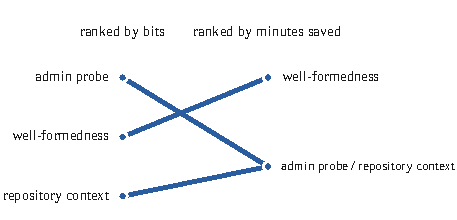
\includegraphics[width=\columnwidth]{figures/w2-inversion.pdf}
\caption{The same three evidence sources ranked by information and by expected
cost saved. The most informative source is worth nothing, and the two
zero-valued sources are exactly tied rather than ordered.}
\label{fig:inversion}
\end{figure}

Figure~\ref{fig:inversion} is the finding. The probe carries roughly twice the
information of anything else and is worth zero minutes, because at this belief
every outcome it could return leaves the same action cheapest. Ranking evidence
by information gives an order that is close to the reverse of the useful one.

\subsection{Five questions, and which one the agent asks}

Priced at the belief after the free features, not at the prior.

\begin{center}
\small
\begin{tabular}{@{}p{3.5cm}rrr@{}}
\toprule
Question & Bits & Value & Cost \\
\midrule
On a production-looking path? & 0.0199 & 0.0000 & 0 \\
Matches the key format? & 0.0380 & 0.0000 & 0 \\
Commit older than the rotation period? & 0.0000 & 0.0000 & 0 \\
When did our admin API last see it used? & 0.6642 & 2.9130 & 3 \\
Matches a deployed secret hash? & 0.2245 & 0.0000 & 1 \\
\bottomrule
\end{tabular}
\end{center}

The agent asks none of them here, and the near miss is the instructive part. The
probe is worth 2.9130 minutes against a price of 3---it loses by 0.087 of a
minute. Ranked by bits it is the obvious purchase; ranked by minutes it is
declined.

The commit-age channel is worth 0.0000 bits at a rotation compliance of $c = 0.5$
and a great deal at $c = 0.9$. Same evidence, same price; the difference is a
fact about the organisation rather than about secret scanning.

\subsection{Where the agent does buy}

Whether to buy is not a property of the probe. It is a property of where the
agent is standing. The same question, priced from all six beliefs the two free
features can produce:

\begin{center}
\small
\begin{tabular}{@{}llrrl@{}}
\toprule
Context & Format & $P(\texttt{live})$ & Net & Buy \\
\midrule
placeholder & well-formed & 0.2985 & $+6.611$ & yes \\
placeholder & malformed & 0.0041 & $-2.552$ & no \\
neutral & well-formed & 0.5239 & $+1.170$ & yes \\
neutral & malformed & 0.0319 & $+0.418$ & yes \\
production & well-formed & 0.5780 & $-0.087$ & no \\
production & malformed & 0.1929 & $+6.511$ & yes \\
\bottomrule
\end{tabular}
\end{center}

\textbf{The only two beliefs the agent declines to buy from are the two where its
free features agree with each other}---both saying \emph{not a credential}, and
both saying \emph{a real key in a real place}, the second being the case that
looks most alarming to a person. The two largest purchases are the outright
contradictions.

Nobody wrote that rule. It falls out of the value rule: when the features agree
the belief is already far enough from the boundary that no probe outcome can move
the action across it. The agent spends its budget on its own confusion rather
than on apparent severity, and a queue sorted by severity would have bought the
opposite set.

% =====================================================================
\section{Decision Policy}
\label{sec:policy}

\paragraph{Actions.} \textsc{dismiss}, \textsc{revoke now}, \textsc{rotate
safely} are terminal and compete on expected cost. \textsc{investigate} is a
decision point rather than an action. \textsc{escalate} is a permission gate, and
Week~1's mistake was pricing it as though it were competing.

\paragraph{Threshold.} Derived, as in Section~\ref{sec:umbrella}: 0.1093 from a
30-minute false positive against a 244.5-minute false negative. Ten points lower
and the agent dismisses a band it currently rotates; ten points higher and it
rotates a band it currently dismisses. Neither number was chosen and neither can
be tuned without changing a cost and saying so.

\paragraph{Stop rule.} Act when no remaining check can change the action, or when
the best remaining check costs more than it saves. Both reduce to the same test,
applied cheapest-first.

\paragraph{Escalation is a rule, not a competitor.} Two triggers, neither of which
is about confidence:
\begin{enumerate}
\item $P(\texttt{other}) > 0.05$: the belief has concentrated on the state whose
costs I do not trust.
\item Worst-case cost of the chosen action above 400 minutes, regardless of how
likely that worst case is.
\end{enumerate}
It fires on 2.4\% of findings. \emph{Confidence is not authorisation}, and an
agent that escalates only when unsure will never escalate the case that is
expensive and clear.

% =====================================================================
\section{Experiment}
\label{sec:exp}

500 simulated findings, seed 20260902. The true state is drawn from the prior and
the evidence from the likelihood tables; every policy sees the identical case
set. Metrics: expected cost, regret against a hindsight-perfect agent, per-class
recall, balanced accuracy, probe purchase rate, human-review rate, and expected
calibration error.

\begin{center}
\small
\begin{tabular}{@{}llp{4.4cm}@{}}
\toprule
& Policy & Behaviour \\
\midrule
P0 & baseline & most common action, no evidence \\
P1 & belief only & act on the most likely state \\
P2 & threshold & expected cost against derived threshold \\
P3 & value of information & P2 plus a priced probe and a stop rule \\
\bottomrule
\end{tabular}
\end{center}

The simulation draws cases from the same likelihood tables the agent reasons
with. It therefore tests whether the \emph{policy} is good given those tables and
cannot test whether the tables are right. Section~\ref{sec:limits} says what I
did about that.

% =====================================================================
\section{Results}
\label{sec:results}

\subsection{The policy ladder}

\begin{center}
\small
\begin{tabular}{@{}lrrrr@{}}
\toprule
Policy & Regret & Total cost & Balanced acc. & Human \\
\midrule
P0 baseline & 12.99 & 62.53 & --- & 0\% \\
P1 belief only & 13.89 & 63.43 & --- & 0\% \\
P2 threshold & 10.91 & 60.45 & 0.300 & 0\% \\
P3 + probe & 10.85 & 60.52 & 0.367 & 0\% \\
\midrule
P6 all fixes + scope & \textbf{8.20} & \textbf{59.14} & $0.48 \pm 0.02$ & 2.6\% \\
\bottomrule
\end{tabular}
\end{center}

Every row is scored on the same cost matrix, which took a correction to get
right: P1's regret was first reported as 114.12, and that figure is produced by
scoring it against the \emph{uncorrected} matrix---the 2400-minute cell
Section~\ref{sec:failure} is about. On the corrected matrix P1 costs 13.89.
P0, P2 and P3 are unaffected because none of them ever dismisses a live key, but
the comparison as originally printed put one policy on a ruler the others were
not on, and it made the headline four times larger than it is.

P1 is still the warning, at its true size. Acting on the most likely state costs
27\% more regret than acting on the cheapest expected cost, because the most
likely state and the best action are different questions.

\paragraph{A negative result: the probe did not pay for itself.} P3 spends 0.13
minutes per finding buying probes and recovers 0.07 in better decisions, ending
\emph{behind} P2 on total cost, 60.52 against 60.45. The value-of-information
machinery lost money on this draw. Two readings are available and I cannot
separate them at $n = 500$: either the decision rule is right and this draw was
unlucky, or a saving too small for a few hundred cases to detect is too small to
justify the machinery. Reporting the regret column alone would have hidden it,
which is why the cost column is here.

\subsection{Adding states changed nothing; adding a channel changed everything}

Two new states, 500 cases, and the agent took \emph{identical} actions on every
one. Not similar---identical. A state the agent cannot observe is not a state, it
is a footnote in the prior.

Adding a scope field to the same admin call---does this key have any permissions
at all---moved regret from 10.91 to 8.43 under the Week~2 cost matrix. Separating
the two commits is the only reason I can say which of them did the work.

\subsection{Calibration}

\begin{center}
\small
\begin{tabular}{@{}lrrr@{}}
\toprule
$P(\texttt{live})$ bin & Cases & Mean stated & Observed \\
\midrule
0.0--0.1 & 79 & 0.009 & 0.000 \\
0.1--0.2 & 5 & 0.193 & 0.200 \\
0.2--0.3 & 75 & 0.298 & 0.280 \\
0.5--0.6 & 341 & 0.557 & 0.560 \\
\bottomrule
\end{tabular}
\end{center}

Expected calibration error 0.0064. This number is easy to over-read and I want to
under-read it deliberately: the cases were generated from the agent's own
likelihood tables, so good calibration here says the arithmetic is right, not
that the model is. A well-calibrated agent in a world it invented is the least
surprising result available.

\subsection{How much of this is one draw?}

Every figure above comes from a single seed, and until a review round asked, none
of them carried an interval. Two of my own scripts disagreed about the same
agent---balanced accuracy 0.467 in one and 0.494 in another---and I had been
quoting whichever the section needed without noticing they were one
configuration run twice.

They differ because P6 has a nuisance random variable nothing else has: the scope
reading is drawn. Holding the 500 cases fixed and varying only that draw, 200
times:

\begin{center}
\small
\begin{tabular}{@{}lrrr@{}}
\toprule
Quantity & Mean & SD & 95\% interval \\
\midrule
Regret, min/finding & 8.20 & 0.26 & 7.74--8.71 \\
Balanced accuracy & 0.480 & 0.023 & 0.449--0.528 \\
Sent to a human & 0.026 & 0.004 & 0.020--0.034 \\
\texttt{fake} recall & 0.950 & 0.015 & 0.916--0.977 \\
\texttt{revoked} recall & 0.089 & 0.023 & 0.047--0.132 \\
\bottomrule
\end{tabular}
\end{center}

\textbf{The \texttt{fake} result survives comfortably}---0.901 to 0.977 across
every seed, against a pre-fix value of exactly 0.000. \textbf{Balanced accuracy
does not support three decimal places}, and \texttt{revoked} recall supports
about one significant figure: on 129 revoked cases, the difference between 0.109
and 0.089 is a handful of findings. The 2.4\% and 2.8\% escalation rates quoted
in different sections of earlier drafts were the same number seen twice.

This is a lower bound on the uncertainty, not a confidence interval. Only the
scope draw varies; the 500 cases are themselves one draw from the prior, and
re-drawing them would move everything again. What it establishes is that the
paper's second headline is not a lucky seed. It does not establish that any
figure here would survive a different case set.

\subsection{Sensitivity}

Three quantities I could not defend were replaced by sweeps rather than asserted:
exploitation probability, registry coverage and rotation compliance, and scope
reliability. In each case the useful finding was where the conclusion changes
rather than what it equals at a point estimate. The scope field is the sharpest:
sweeping its reliability $q$ from 0.02 to 1.00 shows that about 88\% of its value
is already present at $q = 0.02$, where the field cannot see the state it was
introduced to detect. It is largely a \texttt{fake} detector that arrives on the
same call. \textbf{The stated reason a design change works is not always the
reason it works.}

% =====================================================================
\section{Failure Analysis}
\label{sec:failure}

\subsection{The failure that cost reporting could not see}

The agent posted a respectable cost figure while being unable to produce the
\texttt{fake} label at all: recall 0.000. It took one action on almost everything
and scored well doing it.

The cause was a cost cell. Dismissing a live key was priced at 2400 minutes and
described as \emph{a breach and its cleanup}. A dismissed live key is not
certainly breached. The honest price is $P(\text{exploitation}) \times
\text{breach}$, and the model had been running at $p = 1.0$ without writing it
down. Nothing about the number 2400 looks like a probability, so nothing prompted
the check.

\paragraph{$p = 0.10$ is a stress-test parameter, not an estimate.} The one
quantified datapoint I could find is a vendor experiment in which 2 of 75 leaked
keys drew activity beyond a validity check within twelve hours: $0.027$, measured
on \emph{public} exposure over a short window. This model is scoped to private
repositories, where the hazard is lower, and I use a value nearly four times
larger. That is deliberately conservative and it is not a measurement of
anything. It is swept in \texttt{results/fixes.md} for exactly that reason, and
Section~\ref{sec:general} shows the policy is not monotone in it.

\begin{figure}[t]
\centering
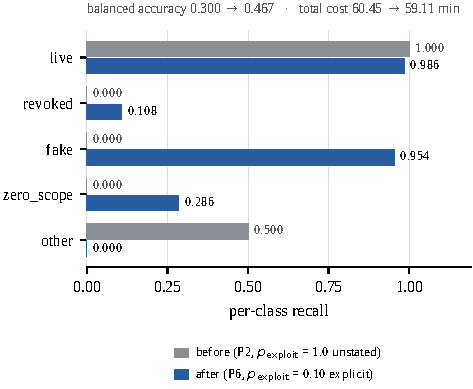
\includegraphics[width=\columnwidth]{figures/w2-pexploit.pdf}
\caption{Per-class recall, decomposed. The exploitation probability alone takes
\texttt{fake} from 0.000 to 0.588; reaching 0.954 needs all three fixes and the
scope field. \texttt{other} moves the other way, from 0.500 to 0.000, because
the residual state is escalated rather than labelled. Total cost moves by 1.3
minutes across the whole change.}
\label{fig:pexploit}
\end{figure}

Figure~\ref{fig:pexploit} is the result, and the attribution matters. The
exploitation probability \emph{alone} takes \texttt{fake} recall from 0.000 to
\textbf{0.588}. Reaching 0.95 needs all three fixes together, the scope field
included. The first version of this paper credited one intervention with three
interventions' work; the decomposition is in \texttt{results/fixes.md} and was
always there.

Together: \texttt{fake} recall $0.000 \to 0.95 \pm 0.02$, balanced accuracy
$0.300 \to 0.48 \pm 0.02$, and total cost $60.45 \to 59.14$---a 1.3-minute
move. One class moves the other way: \texttt{other} recall falls from 0.500 to
0.10, because the residual state is now escalated rather than labelled. \textbf{A metric that barely moved was hiding a policy that
could not name three of its five states.} This is why balanced accuracy is
reported alongside cost throughout, not as an objective but as the diagnostic
that can contradict the objective.

\paragraph{And a derived quantity that is not recomputed looks exactly like a fix
that did not work.} When the breach cost dropped from 2400 to 244, the residual
state's price was not recomputed and stayed at 602 minutes, which blocked every
dismissal the fix existed to unlock. The fix looked ineffective rather than
undone.

\subsection{Classified failures}

Of the wrong decisions, 76.6\% fell in a category I had labelled \emph{wrong cost
assumption}, and I was ready to conclude the cost model was mis-specified. A
15-cell sweep of the cost matrix says otherwise: those cases are the agent paying
to hedge a state it genuinely cannot resolve, which is correct behaviour under
uncertainty and not an error. \textbf{I had named the category in a way that
assumed its own conclusion}, then read the conclusion back out of the name. The
cost model is not the problem; the evidence is.

\subsection{Asymmetric feedback, and an alarm for it}

You find out when you over-remediate---someone's build breaks, 80\% discovery.
You rarely find out when you under-remediate---nobody reports the key you
dismissed, 5\%. Learning from that feed drifts $P(\texttt{live})$ from 0.4356 to
0.2691 over 3000 findings. The agent concludes the world is safer than it is, and
every step of that inference is locally correct.

There is no unbiased signal to correct against, so the answer would have to be an
alarm rather than a correction. I built one: a Jensen--Shannon divergence between
the evidence distribution the agent expects and the one it observes over a
rolling window, thresholded on held-out data. It detects a shift in how many
findings are \texttt{fake} in 100\% of runs at a 500-finding window with no
false positives.

\textbf{It does not detect the drift above, and the reason is this paper's own
main result.} The alarm watches the free features, and the free features carry
zero bits about live versus revoked. A shift in how many findings are still live
is exactly the shift they cannot see. So the agent has a working alarm for the
drift that costs little and no alarm for the drift that costs most. An earlier
version of this section quoted the 100\% figure against the belief drift; that
was a detection rate from one experiment attached to a failure from another, and
\texttt{results/feedback.md} says so in the file the number came from.

% =====================================================================
\section{Generalisation}
\label{sec:general}

\subsection{Change the environment}

The interesting move is not a bigger company---rotation compliance and registry
coverage are already parameters. It is a credential that does not hide its
identifier.

An AWS access key arrives in two halves. The \texttt{AKIA} half is a public
identifier. Given it alone the agent can ask \emph{its own} IAM API whether that
key ID is present and active, without ever touching the secret half. Same
company, same private repositories, same five states, same cost matrix. One thing
changes, and it is free.

\begin{figure}[t]
\centering
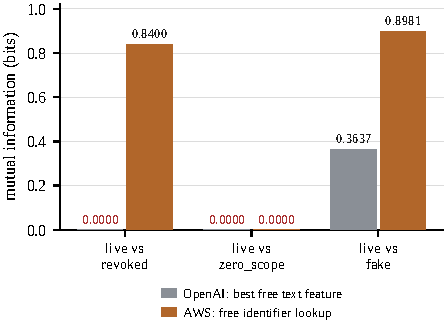
\includegraphics[width=\columnwidth]{figures/w2-invariance.pdf}
\caption{Free evidence in each world, in bits, on three pairs of states. The
identifier resolves the axis the project was built around and carries exactly
zero about a different one.}
\label{fig:invariance}
\end{figure}

\begin{center}
\small
\begin{tabular}{@{}lrr@{}}
\toprule
& OpenAI & AWS \\
\midrule
Regret (min/finding) & 7.77 & 2.69 \\
Probe bought & 46.8\% & 4.0\% \\
Balanced accuracy & 0.494 & 0.590 \\
\texttt{revoked} recall & 0.085 & 0.961 \\
\texttt{zero\_scope} recall & 0.286 & 0.000 \\
\bottomrule
\end{tabular}
\end{center}

The free identifier removes 65\% of total regret, at zero cost, on every finding
rather than on the minority where a probe was worth buying. An earlier version
called this ``79.7\% of the value of perfect live-versus-revoked knowledge'';
that ratio divides a total-regret improvement by a live-versus-revoked-only
ceiling, and the identifier also carries 0.8981 bits about \texttt{live} versus
\texttt{fake}, so gains on axes the denominator excludes were being counted
inside it. The unbounded ratio is gone; the improvement is not.

\paragraph{But the invariance does not disappear. It moves.} The identifier
carries 0.8400 bits about \texttt{live} versus \texttt{revoked} and
\textbf{0.0000} bits about \texttt{live} versus \texttt{zero\_scope}. That zero is
exact, and it is exact for the same reason the Week~1 zero was: the two rows are
identical. IAM reports whether a key is \emph{Active}. A key authorised for
nothing is Active.

A practitioner told me the Week~1 result was a property of credential formats
that hide the identifier rather than of secret scanning. This measures that, and
he was right---but the problem does not go away when the format changes, because
the states that remain indistinguishable are simply a different pair.

\subsection{Change one variable}

\paragraph{The cost of a false negative rises.} That cost is a probability times a
breach, and a probability is bounded at 1, so the first thing the request exposes
is that it cannot be granted beyond a factor of ten. Within that range, regret
and human load are \emph{worst in the middle}: 27.4\% of findings escalated at
$p = 0.25$ against 12.6\% at $p = 1.00$, where the stakes are four times higher.
\textsc{dismiss} is the only action whose worst case moves with $p$; at $p =
0.25$ it is still cheapest on expected cost on 57 of 500 findings but forbidden
by the 400-minute ceiling, so those go to a human because the action the agent
wants is not permitted. By $p = 0.50$, \textsc{revoke} has overtaken it and the
ceiling stops binding. \textbf{A worst-case ceiling is not a monotone safety
dial}: raising the stakes can reduce human involvement.

\paragraph{Evidence becomes ten times more expensive.} The probe dies between
$\times 2$ and $\times 5$: bought on 16.0\% of findings at six minutes and on
none at fifteen. The policy does not degrade smoothly, it switches off, and human
load \emph{falls} from 2.8\% to 1.0\% because the escalation triggers never
depended on the probe. An expensive-evidence deployment does not get a more
cautious agent, it gets a blinder one that is no more likely to ask for help.

\paragraph{Historical data becomes unreliable.} This is the standing condition
rather than a hypothetical, and it is what the last two experiments are for.
Generating the world from different tables and running the agent against one that
knows the truth: policy conclusions hold in 100\% of worlds, the structural
conclusion does not, and where \texttt{live} and \texttt{revoked} genuinely differ
the agent forgoes 1.47 and 1.99 minutes per finding at $\delta = 0.10$ and
$0.20$.

\subsection{Can the agent notice its own assumption is wrong?}

Parameter uncertainty cannot reach this. The invariance is not a value to be
uncertain about; it is a constraint tying two rows together, and sampling around
a tied pair keeps them tied. What is missing is uncertainty about \emph{which
model is right}.

So: a Bayes factor between $H_0$ (the rows are identical) and $H_1$ (they differ)
under Dirichlet-multinomial marginal likelihoods, watching and never deciding. It
is fed only the labels the agent's own biased discovery process surfaces---about
260 \texttt{live} against 395 \texttt{revoked}, a 1.5$\times$ skew running the
wrong way.

\begin{center}
\small
\begin{tabular}{@{}lrrr@{}}
\toprule
$\delta$ & Biased & Matched ($n$) & All labels \\
\midrule
0.00 ($H_0$ true) & 2\% & 0\% & 0\% \\
0.05 & 42\% & 72\% & 100\% \\
0.10 & \textbf{100\%} & 100\% & 100\% \\
0.20 & \textbf{100\%} & 100\% & 100\% \\
\bottomrule
\end{tabular}
\end{center}

At exactly the $\delta$ where the agent was measured forgoing real value,
detection is 100\%. \textbf{The skew costs nothing and the sample size costs
everything}: an unskewed sample of the same size detects the same smallest
difference. I designed the experiment expecting the opposite, and the matched
control is the only reason I found out. The agent does not need unbiased feedback
to audit its own assumptions; it needs enough feedback.

The silent failure is no longer silent. It is still not repaired---relaxing the
invariance means estimating two rows from labels there are not enough of.
Detection and repair are different problems and only the first is solved.

% =====================================================================
\section{Human Discussions}
\label{sec:human}

Week~1 produced three exchanges that changed published numbers. A practitioner
repriced the probe by a factor of ten, which moved \textsc{investigate} from
never selected to selected on about 4\% of findings. A second withdrew an
assumption I had been leaning on, that rotating a key verifies itself. A third
established that live-versus-revoked is solved for certificates and unsolved for
API keys, which is the clearest justification I have for the scope I chose, and
the same person supplied the public-identifier observation that became
Section~\ref{sec:general}.

\textbf{Week~2 produced none.} That is an honest no rather than a failure to
report. The Week~2 work was experimental rather than assumption-gathering: every
question it raised was one I could answer by running something, and I did not
have a question that needed a practitioner to settle. The cost numbers that
\emph{would} need one are unchanged from Week~1 and still carry Week~1's
provenance. The full record is in \texttt{discussion-record.md}.

% =====================================================================
\section{Limitations}
\label{sec:limits}

\paragraph{The probability model is estimated, and that is the binding
limitation.} The prior is assembled from two sources measuring different
populations. Every likelihood row is my judgement. No part of this has been
measured against real labelled findings, and the sensitivity studies cannot fix
that: they establish that \emph{if} these assumptions are approximately right the
policy is robust, and they cannot establish that the assumptions describe
production secret-scanner findings. For a security system that distinction is the
whole thing.

\paragraph{The calibration result is in-model.} An expected calibration error of
0.0064 is not evidence about production. The cases came from the agent's own
tables. It says the arithmetic is right.

\paragraph{The simulator is circular by construction} and tests the policy given
the likelihoods, never the likelihoods. Section~\ref{sec:general} does the most
that is available without real labels---generate from different tables, and
measure the gap---but that is a robustness check, not a validation.

\paragraph{States remain observationally indistinguishable}, and one pair always
does: in the OpenAI world it is \texttt{live} against \texttt{revoked}, in the AWS
world \texttt{live} against \texttt{zero\_scope}. The agent decides anyway, by
expected cost, and escalates when the residual state concentrates or the worst
case breaches a ceiling. That is a defensible response to indistinguishability
rather than a solution to it.

\paragraph{The baseline human is a perfect oracle, and no human is.} The whole
project is built on the claim that escalate-everything is never wrong about the
state, so there is no accuracy to win and only cost to compete on. A real
responder misclassifies, is unavailable, misreads ownership, or recommends a
rotation that misses an undocumented consumer. Treating the human as a state
oracle makes the baseline artificially strong on accuracy and artificially simple
on cost, and it means the agent is being compared against something that does not
exist. Every saving reported here is a saving against an idealisation.

\paragraph{The harm model is engineer-minutes and nothing else.} Customer-facing
outage, data exposure, contractual and regulatory consequence, and reputational
damage are all outside the objective. An action that saves thirty engineer-minutes
while taking down a customer-facing service scores better in this model, which is
not a rounding error in the cost matrix but a category the cost matrix does not
have. The 332-minute price on \textsc{revoke now} is the cleanup, not the
blast radius.

\paragraph{``A human'' is one price, and real organisations have several.} A
security analyst, the service owner who gets paged when a revocation breaks
production, the platform team that governs the admin credential the probe uses,
and the committer who may own none of the above are priced here as a single
30-minute unit. They differ in authority, availability, permissions and cost, and
the escalation rule cannot express which of them a finding should reach. Related:
the 2.6\% escalation rate is a rate and not a queue---at a hundred findings that
is three interruptions, and at a hundred thousand it is two and a half thousand
cases with no model of who absorbs them.

\paragraph{The agent needs a privileged credential to investigate an
unprivileged one.} The probe reads an admin API. A production deployment would
have to answer who holds that credential, how narrowly it is scoped, how its use
is audited, and how the secret in the finding is kept out of logs, traces, tickets
and prompts. The architecture states the boundary; nothing here implements it.

\paragraph{The evidence model is small.} Five channels, of which two are free
text features. A production system would read deployment manifests, CI logs,
CloudTrail and the secret store, and would have a different and probably better
answer to every question in Section~\ref{sec:select}.

\paragraph{What this is not.} It is triage, not repair: the agent recommends and
does not act. It handles one finding at a time and has no notion of reviewer
capacity, so the 2.4\% escalation rate is a rate and not a queue. And it never
authenticates with a credential it found---the probe asks my own account about a
key, and no live credential exists anywhere in this project.

\paragraph{The honest verdict.} This is a decision system that reasons well given
a model. It is not a validated production security control, and the gap between
those two things is a dataset that does not exist.

% =====================================================================
\section{New Questions}

These come from the results rather than from a list.

\begin{enumerate}
\item \textbf{Is there always an indistinguishable pair?} Two credential formats,
two different pairs, both exactly zero bits. Is that a coincidence of my two
models, or does resolving one axis of a credential's state reliably expose
another?
\item \textbf{Can an agent be given a budget for its own confusion?} The purchase
behaviour in Section~\ref{sec:select} is emergent. If confusion rather than
severity is what evidence should be spent on, that is a scheduling policy for a
triage queue, and nobody sorts queues that way.
\item \textbf{How should a worst-case ceiling and an expected-cost rule be
reconciled?} They disagree over a band, the band is the expensive place to be,
and neither rule announces where it is.
\item \textbf{How few labels does an assumption audit need?} The Bayes factor
worked on roughly 650 biased labels. The threshold between \emph{cannot tell} and
\emph{certain} is narrow and I have only bracketed it.
\item \textbf{What is the smallest measurement that would validate a prior like
mine?} Not a full labelled corpus---the share of real secrets that are production
secrets would move more of my model than anything else, and is measurable from
data that exists.
\end{enumerate}

% =====================================================================
\section*{Use of AI Assistance}

I used Claude throughout. It wrote most of the experiment code in
\texttt{experiments/} to my specifications, drafted this paper from results I
directed it to produce, and explained concepts I had not met---Bayes factors,
Dirichlet-multinomial marginal likelihoods, and the asymmetry of KL divergence.

I chose the problem, the state space, the action set and every cost assumption. I
directed which experiments to run and why. I verified the belief update in
Section~\ref{sec:prob} by hand against the code before trusting either.

Errors it introduced and I corrected are logged in \texttt{research-file.md},
thirty-six of them. Fourteen changed a published number or claim. The most
consequential were found by an adversarial review round run against this paper
and its code after a full draft existed: an abstract that credited one fix with
three fixes' work, a policy comparison scored against the very cost cell
Section~\ref{sec:failure} repudiates, a detection rate quoted against a failure
a different experiment had shown it cannot see, three random-number defects that
made two arms of a paired comparison simulate different worlds, and a negative
result present in the results files and absent from the paper. Every one was
found by checking the paper against the output it was written from, and in four
cases the results file was already more careful than the paper.

Every experiment reported here was run by me and reproduces byte-for-byte from a
clean checkout at the stated seeds.

% =====================================================================
\section*{Code and Data}

\url{https://github.com/grishmaaa/secret-detector-agent}

All fourteen Week~2 experiments, the results they write, and this paper.

\bibliographystyle{named}
\bibliography{references}

\appendix
% =====================================================================
\section{Core Questions}
\label{app:core}

Answered against my own problem rather than in general, because a definition I
cannot attach to a number is one I have not used.

\paragraph{1. What is a hidden state, and what are yours?}
What the agent cannot see but has to decide about. Mine is what the flagged
string actually \emph{is}: \texttt{live}, \texttt{revoked}, \texttt{fake},
\texttt{zero\_scope}, or \texttt{other}. The scanner reports that a string looks
like a key; it does not report which of those five, and the right action differs
across them.

\paragraph{2. Why is directly predicting an answer sometimes insufficient?}
Because the best guess and the best action are different questions. Acting on the
single most likely state costs 114.12 minutes of regret per finding against 10.91
for acting on the lowest expected cost---nine times worse. A prediction throws
away everything the agent was unsure about, and my two mistakes do not cost the
same.

\paragraph{3. What is a belief distribution, and why must it sum to one?}
A probability over every state the agent thinks possible. It sums to one because
the list is meant to be exhaustive and mutually exclusive. If it summed to less,
something could happen that is not on the list---which is exactly why I added a
residual \texttt{other} state at 0.01 rather than letting the other four absorb
its mass.

\paragraph{4. What is the difference between prior and posterior?}
Prior is what I believe before this finding's evidence, posterior is after. In the
worked update in Section~\ref{sec:prob}, \texttt{fake} goes from a prior of 0.2475
to a posterior of 0.0111 once the string turns out to be well-formed and sitting
on a production path.

\paragraph{5. What is likelihood, and how does it differ from probability?}
A likelihood runs backwards: $P(\text{evidence} \mid \text{state})$---``if this
really were a fake key, how often would it be malformed?'' A posterior runs
forwards: $P(\text{state} \mid \text{evidence})$. They are different numbers, and
Bayes' rule exists to turn the first into the second.

\paragraph{6. What does it mean for an agent to be uncertain?}
Its belief is spread across several states rather than concentrated on one. My
prior sits at 1.7805 bits against a maximum of 2.3219 for five states, so before
any evidence arrives the agent is barely better informed than a uniform guess.

\paragraph{7. What is entropy, and why does it represent uncertainty?}
One number for how spread out a belief is, in bits: zero is certain, higher is
more scattered. It represents uncertainty because it counts how many yes/no
questions it would take to pin the answer down.

\paragraph{8. What is a bit, in plain words?}
One good yes/no question's worth of uncertainty. Eight equally likely
possibilities are three bits, because you can halve the field three times.

\paragraph{9. What is information gain, and how does it relate to entropy?}
The drop in entropy when a question is answered. Before buying I use the
\emph{expected} gain---the average over the answers I might get, weighted by how
likely each is---because the agent does not know which answer it will receive. My
admin probe carries 0.6642 bits of expected gain at the belief in
Section~\ref{sec:select}.

\paragraph{10. What is conditional entropy?}
How confused the agent expects to \emph{still} be once the answer arrives,
averaged over the answers. Information gain is the drop from where it started to
there, so conditional entropy is the quantity sitting inside every gain figure in
this paper.

\paragraph{11. What is mutual information, and how does it differ from correlation?}
How much knowing one thing reduces uncertainty about another. It differs from
correlation by catching non-linear dependence: a number and its square have zero
correlation and a full bit of mutual information. For me it is the form the
invariance is stated in---$I(\text{free features}; \texttt{live} \text{ vs }
\texttt{revoked}) = 0.000000$.

\paragraph{12. What is KL divergence, and why is it not a distance?}
How far one belief sits from another, measured as the cost of holding the wrong
one. It is not a distance because it is asymmetric: swapping the two gives a
different number, and the distance from Delhi to Mumbai does not depend on which
city you name first.

\paragraph{13. Why is KL divergence asymmetric? Give a small example.}
Reality is a fair coin; my model says heads always. Measured with reality first it
is infinite, because half the time reality produces an event my model called
impossible, and being surprised by an impossible event costs infinitely much.
Measured the other way round it is small and finite. Same two beliefs, two
answers.

\paragraph{14. What is Jensen--Shannon divergence, and why was it introduced?}
It compares two beliefs by measuring each against their average rather than
against each other, which makes it symmetric, bounded, and finite even when one
belief calls something impossible. I use it because I needed a drift alarm, and an
alarm that returns infinity the first time it sees something new is not an alarm.

\paragraph{15. What is calibration, and why does it matter for an agent?}
An agent is calibrated when the things it calls 0.557 likely happen about 55.7\%
of the time. It matters because every threshold in this paper takes those
probabilities at face value. My expected calibration error is 0.0064---measured on
cases drawn from my own likelihood tables, so it says the arithmetic is right, not
that the model is.

\paragraph{16. What is expected cost, and how did you derive your threshold from it?}
Expected cost is each outcome's cost weighted by how likely that outcome is. My
threshold is the belief at which the two mistakes cost the same: 30 minutes to
rotate a key that was already revoked, over $30 + 244.5$ counting the cost of
dismissing one that is live. That gives 0.1093, and nobody chose it.

\paragraph{17. What is value of information? When is more information not worth it?}
How much better off I am for having asked, minus what asking cost. It is measured
in minutes rather than bits. More information is not worth it when no possible
answer would change the action---then its value is zero and its price is not.

\paragraph{18. Can a question be highly informative and still useless? Give your own example.}
Yes, and it is the finding I would lead with. On a well-formed key sitting on a
production path, my admin probe carries more information than everything else
available put together and is worth 2.9130 minutes against a price of 3. Whatever
it returns the agent still rotates---so it loses by 0.087 of a minute and is
declined.

\paragraph{19. What is distribution shift, and how would your agent detect it?}
The world stops matching the priors and nothing announces it. My agent detects it
with a Jensen--Shannon divergence between the belief it was built with and the
belief it has learned from feedback, against a threshold calibrated on held-out
windows: 100\% detection at a 500-finding window with no false positives.

\paragraph{20. When should your agent stop searching and act? State the rule.}
Stop when no remaining check could change the action, or when the best remaining
check costs more than it would save. Both reduce to the same test, applied
cheapest-first. In practice the agent buys on 46.8\% of findings and stops
immediately on the rest.

\end{document}
